\documentclass[11pt]{article}
\usepackage{amsmath}
\usepackage[margin =1 in]{geometry}
\usepackage{bm}
\usepackage{graphicx}
\usepackage{times}
\usepackage{rotating}
%\usepackage[pdftex]{hyperref}
\usepackage{hyperref}
\usepackage{setspace}
\newcommand{\overbar}[1]{\mkern 1mu\overline{\mkern-1mu#1\mkern-1mu}\mkern 1mu}
\usepackage[usenames,dvipsnames]{xcolor}
\definecolor{rose}{rgb}{1.0, 0.01, 0.24}
\definecolor{blue}{rgb}{0.0, 0.0, 1.0}
\definecolor{green}{rgb}{0.0, 1.0, 0.0}
\definecolor{orange}{rgb}{1,0.5,0}
\definecolor{violet}{rgb}{0.58, 0.0, 0.83}
\def\green#1{\textcolor{green}{#1}}
\def\blue#1{\textcolor{blue}{#1}}
\def\red#1{\textcolor{red}{#1}}
\def\orange#1{\textcolor{orange}{#1}}
\def\violet#1{\textcolor{violet}{#1}}


\begin{document}
\onehalfspacing

\title{Mini Project IV \\
Clustering Texts} 
\author{Arthur Lui \and Jared Ward}

\maketitle

\section*{Introduction}
Recent interest in identifying authorship of written text by analytical analysis
has opened the doors to some interesting research in this arena. In this study,
we compare categorical clusterings of texts by genre to unsupervised
clusterings. These unsupervised clusterings are created through summary
statistics that summarize writer styles. We have 18 indicators of style,
including how much an author writes in first person, the motion or spacing of
the text, and others.  Jeff Collins
\footnote{https://tofu.byu.edu/stat666/assignments/DissertationOn18RhetoricalCategories.pdf}
study on textual analysis contains a more complete listing of the variables used
and how they are quantified. 
\\
\\
We have 1000 texts with 15 common genres for which these texts fall under. We
wish to analyze how natural groupings compare to the way the texts are currently
classified, as well as compare how 5 clusters grouped naturally compare to 5
"super genres" comprising the following: Press, Non-press Nonfiction, Biography,
Scholarship and Official Documents, Fiction. 
\\
\\
How well do authors styles within a genre categorize texts? Do Authors writing
styles stick to genre or is there significant overlap? This analysis will help
uncover some statistics governing these phenomenon.  

\section*{Clustering the Texts}
We begin by clustering the texts into groups of 3,4,5,6, and 7. That is, we
create 3 clusters of the 1000 texts, then a separate 4 clusters, and so on to 7.
The clusters are initially created using Ward's Linkage, then bettered using an
iterative algorithm called k-means.

\subsection*{Ward's Linkage}
There are a variety of ways to create clusters. One reasonable method to get
clusters is using Ward's Linkage. This method begins by clustering the two
points nearest in Eulidean distance. The algorithm then considers the next two
closets points, treating the centroid of the pair just created as a point. So if
the two nearest points of the data (including the pair made in the last step) is
the centroid of the couplet just created and another point, the cluster created
in the first step becomes a triplet. Otherwise, another couplet is formed, and
the centroid is treated as a "point" when creating the next cluster. This
process is iterated until a predetermined number of clusters are created. 

\subsection*{K-means}
Another way to calculate clusters is using the k-means method. K-means creates
clusters by moving observations across groups until the sums of squares of
Euclidean distances for each observation to its group mean. The process begins by
selecting an initial set of clusters. Observations are then moved to the group
with the nearest centroid (using the Euclidean distance metric). Centroids
are recalculated, and the process repeats until none of the observations move
to different clusters.
\\
\\
A criticism of this method is that initial starting groups need to be selected,
and different starting groups don't necessarily converge to the same final
groups. To utilize this idea of maximizing distance between groups, some propose
beginning with multiple sets of random starts then choosing the best set of
final groups. We instead use Ward's Linkage to get a reasonable starting set of
groupings, and better the classification of observations into groups by using
the k-means algorithm.

\subsection*{Selecting the Best Set of Clusters}
Now we have a best set of clusters for k$=$3,4,5,6, and 7 clusters. Choosing how
many clusters we should use is a somewhat subjective procedure. We first conduct
a MANOVA test of the following form: 
\\
\indent $H_0$: There is no difference of means: $\bf{\mu}_{1} = \bf{\mu}_{2} =
... = \bf{\mu}_{k}$ Vs.
\\
\indent $H_0$: At least one $\bf{\mu}_{j}$ is different from the others: $\bf{\mu}_{j} \ne \bf{\mu}_{i}$ for some $i \ne j$
\\
where k is the number of clusters, $\bf{\mu}_{j}$ is the cluster mean for the $j^{th}$ cluster, and $i$, $j$ $\in$ 1,...,k.
\\
\\ 
However, in each case the null hypothesis is rejected with $p<.0001$. This is
expected as we hope the clustering are statistically different. As a second
selection method, we look at misclassification rates for each set of clusters.
This is done by calculating the best clusters, then (using the same calculating
procedure) recalculating clusters holding out one observation. 
\\
\\
Once new clusters are obtained, we then see if the hold-out observation is
predicted back into the same group it was originally a part of, i.e. is the
observation still closest to the mean of the original cluster it was in. If this
is not the case, we say this point has been misclassified. This method
demonstrates the stability of the clusters. We repeat this process for all 1000
data points and calculate the percentage misclassified for each of the clusters
of 3,4,5,6, and 7. The results are included in the following table.

\input errRate.tex

\noindent Cluster 3 has the lowest misclassification rate. We would expect
grouping to be more distinct for smaller sets of groups, and in fact we see that
misclassification rates increase with number of clusters. This procedure is
again somewhat objective, but group 3 seems to have a much lower
misclassification rate than other groups, so we choose $k=3$.

\section*{Attributes of Clusters}
Our clusters live in $s-space$ defined by $min(p,k-1)$ where $p$ is the number
of variables in each observation (18) and $k$ is the number of clusters (3). So
$s=2$. This implies there is a plane that spans the space of best separation for
the group means, unless their means are somewhat collinear in which case the
plane that best separates the means can be collapsed to essentially a line. The
non-zero eigenvalues of $E^{-1}H$ are 4.028 and 1.119. 
\\
\\
This implies $\lambda_1$ and the corresponding eigenvector contains 78.25 percent
of the variation of the plane in one direction. This certainly means there is
more separation in one direction than in the perpendicular direction defined by
$\lambda_2$ and the corresponding eigenvector. But we need this 2-D plane to span 
the space of best separation.

\input EH.tex

\noindent  More extreme measurements of the variables measured corresponding to
the bolded components for each eigenvector are going to best separate texts in
each direction of the plane respectively. 
\\
\newpage
\noindent Groups are best separated by the plane created in the two orthogonal
directions as the eigenvectors listed above. This is graphically is illustrated
by the following plot.

\begin{center}
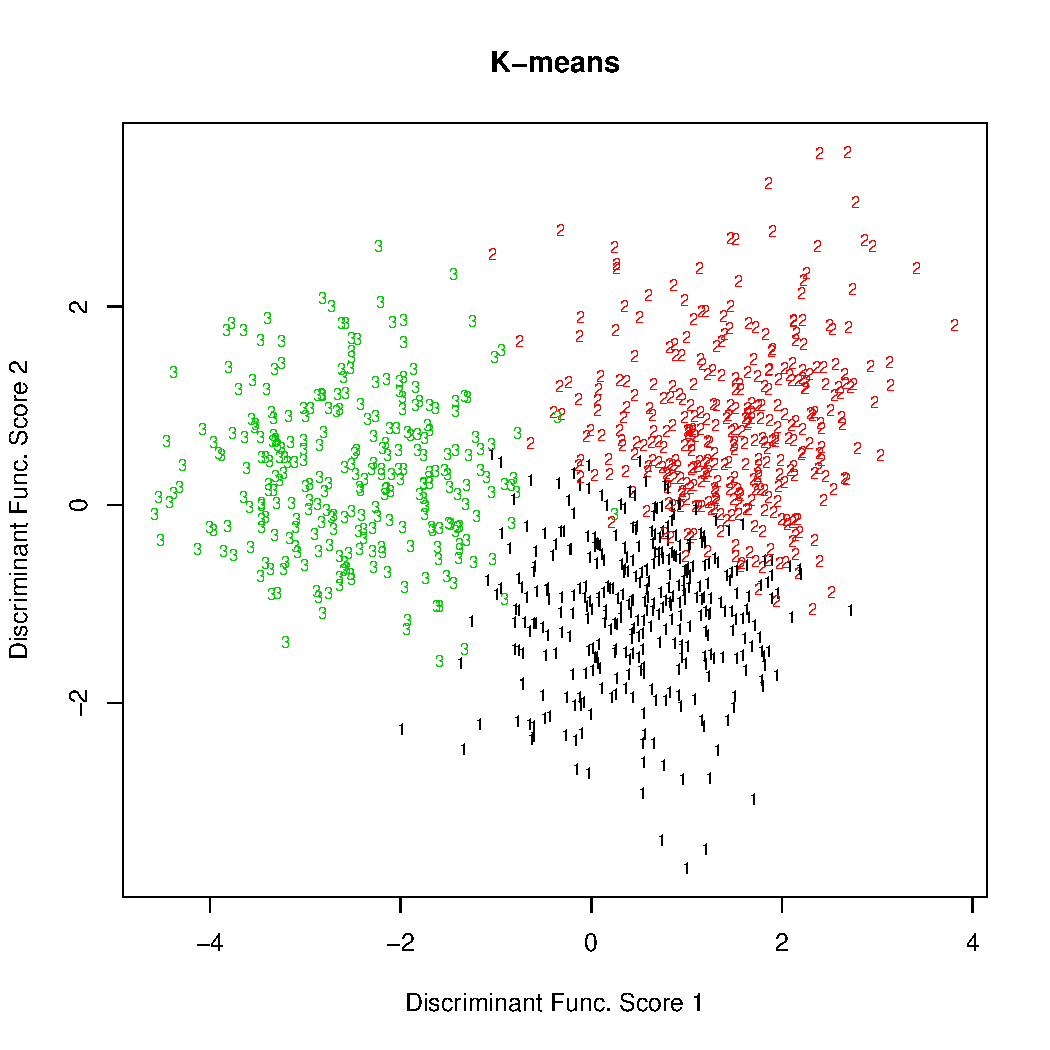
\includegraphics[width=.5\textwidth]{disc.pdf}
\end{center}

\noindent Note the table below that shows which proportion of the 15 genre's
were put into each of the 3 groups. 

% latex table generated in R 3.0.2 by xtable 1.7-1 package
% Thu Nov 20 07:18:46 2014
\begin{table}[ht]
\centering
\begin{tabular}{rrrr}
  \hline
 & Cluster 1 & Cluster 2 & Cluster 3 \\ 
  \hline
Press: Reporting & \bf{0.86} & 0.11 & 0.02 \\ 
  Press: Editorial & 0.17 & \textcolor{rose}{0.80} & 0.04 \\ 
  Press: Reviews & \bf{0.79} & 0.18 & 0.03 \\ 
  Religion & 0.09 & \textcolor{rose}{0.88} & 0.03 \\ 
  Skills and Hobbies & \bf{0.67} & 0.29 & 0.04 \\ 
  Popular Lore & 0.42 & 0.49 & 0.09 \\ 
  Biography & 0.33 & 0.51 & 0.16 \\ 
  Official Communications & 0.53 & 0.47 & 0.00 \\ 
  Learned & 0.40 & 0.59 & 0.01 \\ 
  General Fiction & 0.02 & 0.02 & \textcolor{green}{0.97} \\ 
  Mystery & 0.02 & 0.00 & \textcolor{green}{0.98} \\ 
  Science Fiction & 0.00 & 0.08 & \textcolor{green}{0.92} \\ 
  Adventure & 0.03 & 0.00 & \textcolor{green}{0.97} \\ 
  Romance & 0.02 & 0.02 & \textcolor{green}{0.97} \\ 
  Humor & 0.06 & 0.06 & \textcolor{green}{0.89} \\ 
   \hline
\end{tabular}
\end{table}

\noindent Notice that texts for some of the genre's fall predominately into one
cluster.  In some sense, our natural clusters have classified some genre's
primarily into one cluster, and further, similar genre's have been grouped
together. Cluster 3 seems to be the fiction genre, while clusters 1 and 2 seem
to make up the other genres. Perhaps clusters 2 contains more objective
non-fiction, and cluster 1 the somewhat subjective non-fiction.

\section*{Comparing Super Genres}
We now want to see how the 5 super genres compare to the 5 natural clusters
created above. A comparison of misclassification rates for each grouping, (the
super genres and natural clusters for k$=$5), as well as some intuition into
how these genres in general are being grouped will be outlined.
\\
\\
Super Genres have a higher misclassification rate (.36) than that of the
natural clusters (.24) for k=5 (see Table 2). A MANOVA reveals that the
centroids of super genres and natural clusters are both significant, but the
natural centroids are more distinct than the super genre centroids. The
F-statistics are 83.6 and 35.3 respectively (see Table 3). From a heat map of
the proportions of super genres to natural clusters, it appears that the fourth
\& fifth clusters combine to form the Fiction genre. And Clusters 1 to 3 make
up the non-fiction genre.

\input errVS.tex     % Table 2
\input compSupK5.tex % Table 3

%\begin{center}
%  \textbf{Proportions of Super Genres Vs. Natural Clusters}
%  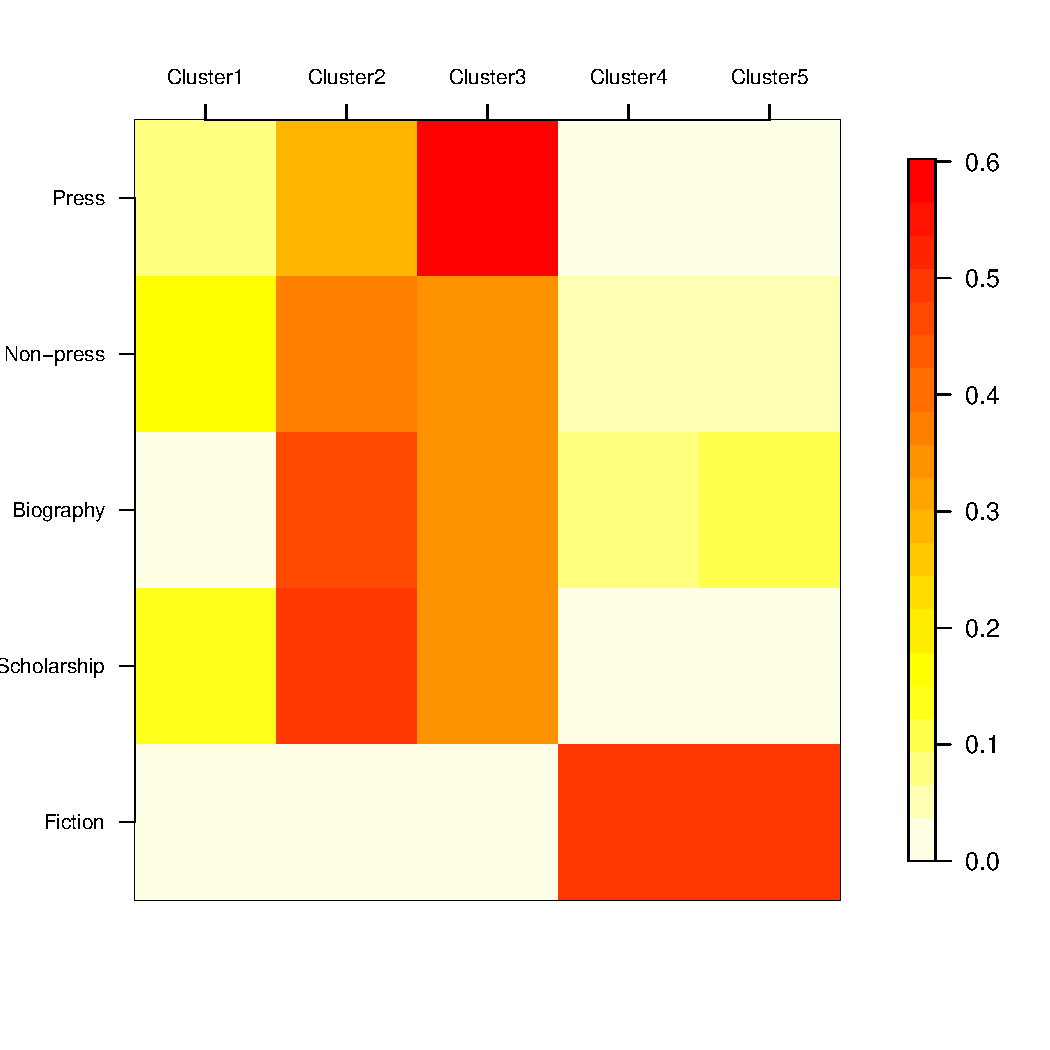
\includegraphics[scale=.5]{supK5prop.pdf}
%\end{center}

\begin{center}
  \textbf{Proportions of Genres Vs. Natural Clusters}\\
  %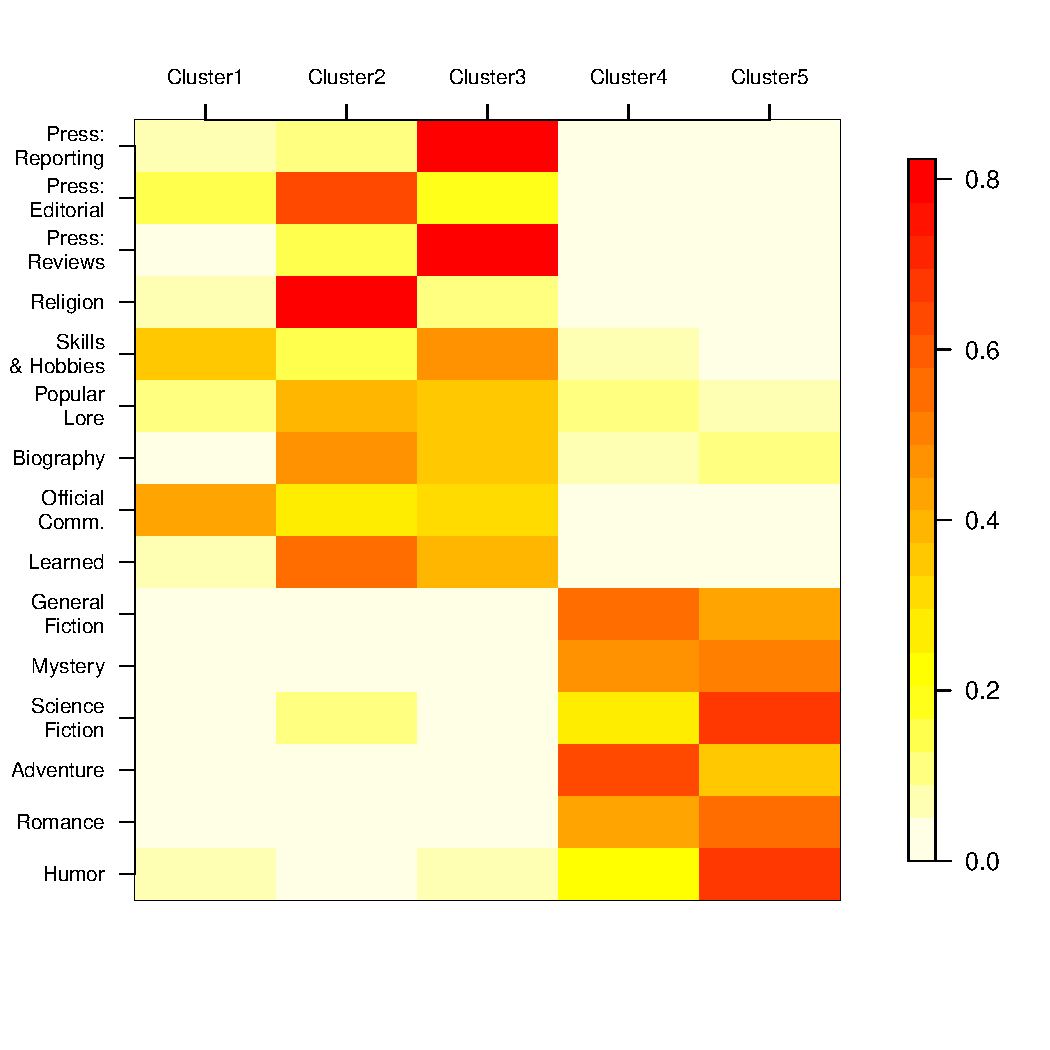
\includegraphics[scale=.5]{15by5.pdf}
  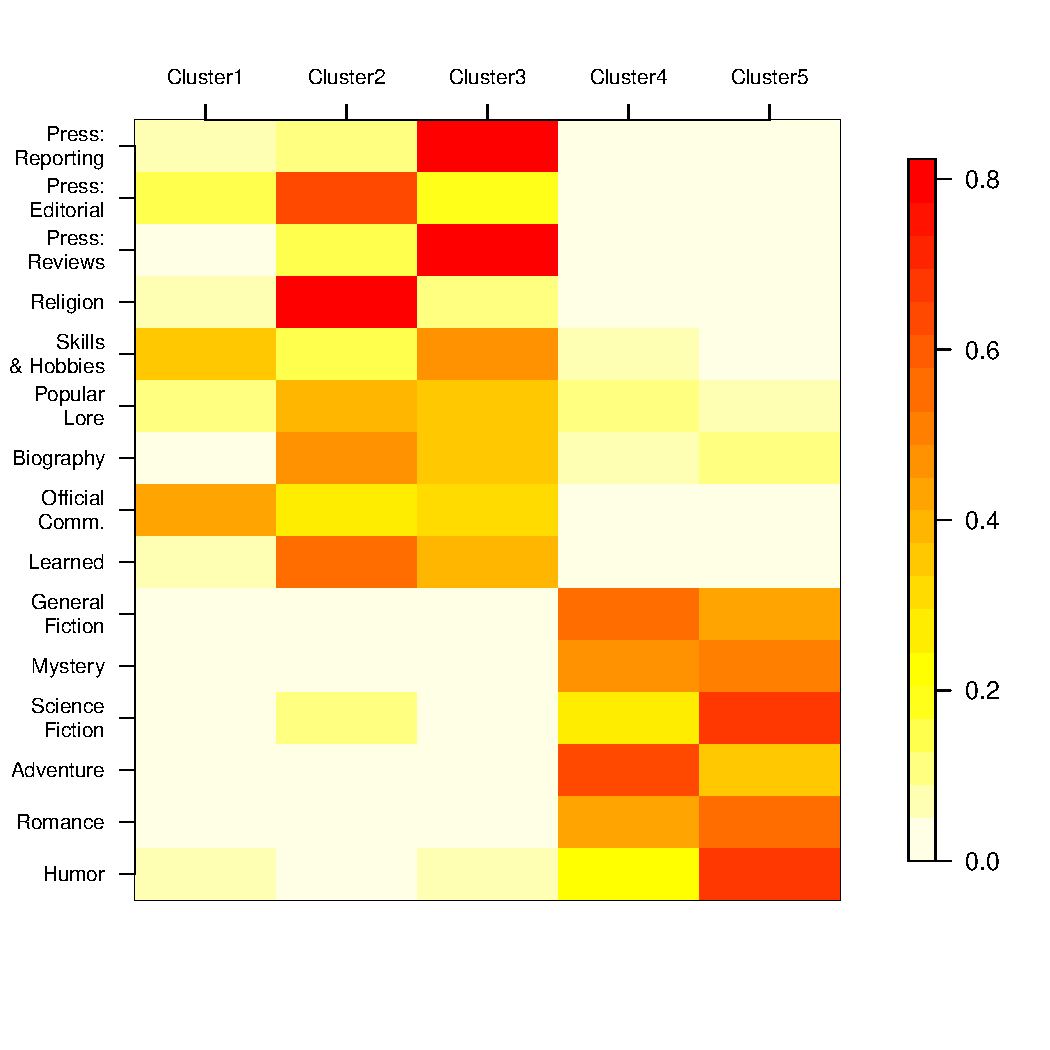
\includegraphics[scale=.5]{join.pdf}
\end{center}

\section*{Conclusion}
We determined the ward linkage performs the best for separating our data into 
different clusters. The optimal number of clusters, is 3. That is, separating 
our data into three clusters yields the lowest misclassification rate. 
Natural cluster means and super genre means are significantly different.
It appears that there are 2 main clusters - fiction and non-fiction. 
The non-fiction genres can also be subdivided into subjective and non-subjective 
writing. Subjective writing includes religion and editorials; non-subjective 
writing includes reporting and reviews.

\end{document}
